\chapter{THỰC THI KIỂM THỬ VÀ QUẢN LÝ LỖI TRÊN MANTIS}

\section{Thiết lập môi trường và Thực thi kiểm thử}

\subsection{Môi trường thực thi kiểm thử}
Quá trình kiểm thử website cửa hàng tiện lợi 7coMART được thực thi trên môi trường máy chủ cục bộ đồng bộ hóa bằng Docker Compose với các cấu hình phần mềm cụ thể sau:
\begin{itemize}
    \item \textbf{Địa chỉ ứng dụng:} \url{http://localhost} (Cổng HTTP chuẩn được phục vụ bởi Nginx Reverse Proxy).
    \item \textbf{Địa chỉ API Backend:} \url{http://localhost:8000/docs} (Swagger UI phục vụ gọi test API độc lập).
    \item \textbf{Hệ điều hành kiểm thử:} Microsoft Windows 11 Enterprise.
    \item \textbf{Trình duyệt sử dụng:} Google Chrome (Version 122 ổn định) kết hợp công cụ Chrome Developer Tools (F12) để theo dõi luồng mạng Network Tab và ghi nhận lỗi JavaScript Console.
\end{itemize}

\subsection{Quy trình và Quy ước ghi nhận kết quả thực thi}
Tester tiến hành duyệt qua từng kịch bản kiểm thử đã định nghĩa ở Chương 2, thao tác trực tiếp trên giao diện người dùng và tiến hành đối chiếu Kết quả thực tế (\textit{Actual Result}) với Kết quả mong đợi (\textit{Expected Result}). Trạng thái của kịch bản test được đánh giá theo quy ước:
\begin{itemize}
    \item \textbf{Đạt (Pass - P):} Khi hệ thống phản hồi chính xác, Kết quả thực tế trùng khớp hoàn toàn với Kết quả mong đợi.
    \item \textbf{Lỗi (Fail - F):} Khi hệ thống phản hồi sai logic nghiệp vụ, phát sinh lỗi Crash trang, lỗi 500 API hoặc xuất hiện lỗ hổng bảo mật nghiêm trọng. Mọi ca kiểm thử mang trạng thái Fail đều bắt buộc phải được lập báo cáo lỗi (Defect Report) và đẩy lên hệ thống quản lý lỗi trực tuyến Mantis Bug Tracker.
\end{itemize}

\subsection{Minh họa giao diện thực thi kiểm thử các Sprints}
Dưới đây là một số hình ảnh chụp màn hình ghi nhận giao diện thực tế của website 7coMART trong quá trình nhóm tiến hành thực thi kiểm thử thủ công cho Sprint 1 và Sprint 2:

\begin{figure}[H]
    \centering
    \begin{minipage}{0.48\textwidth}
        \centering
        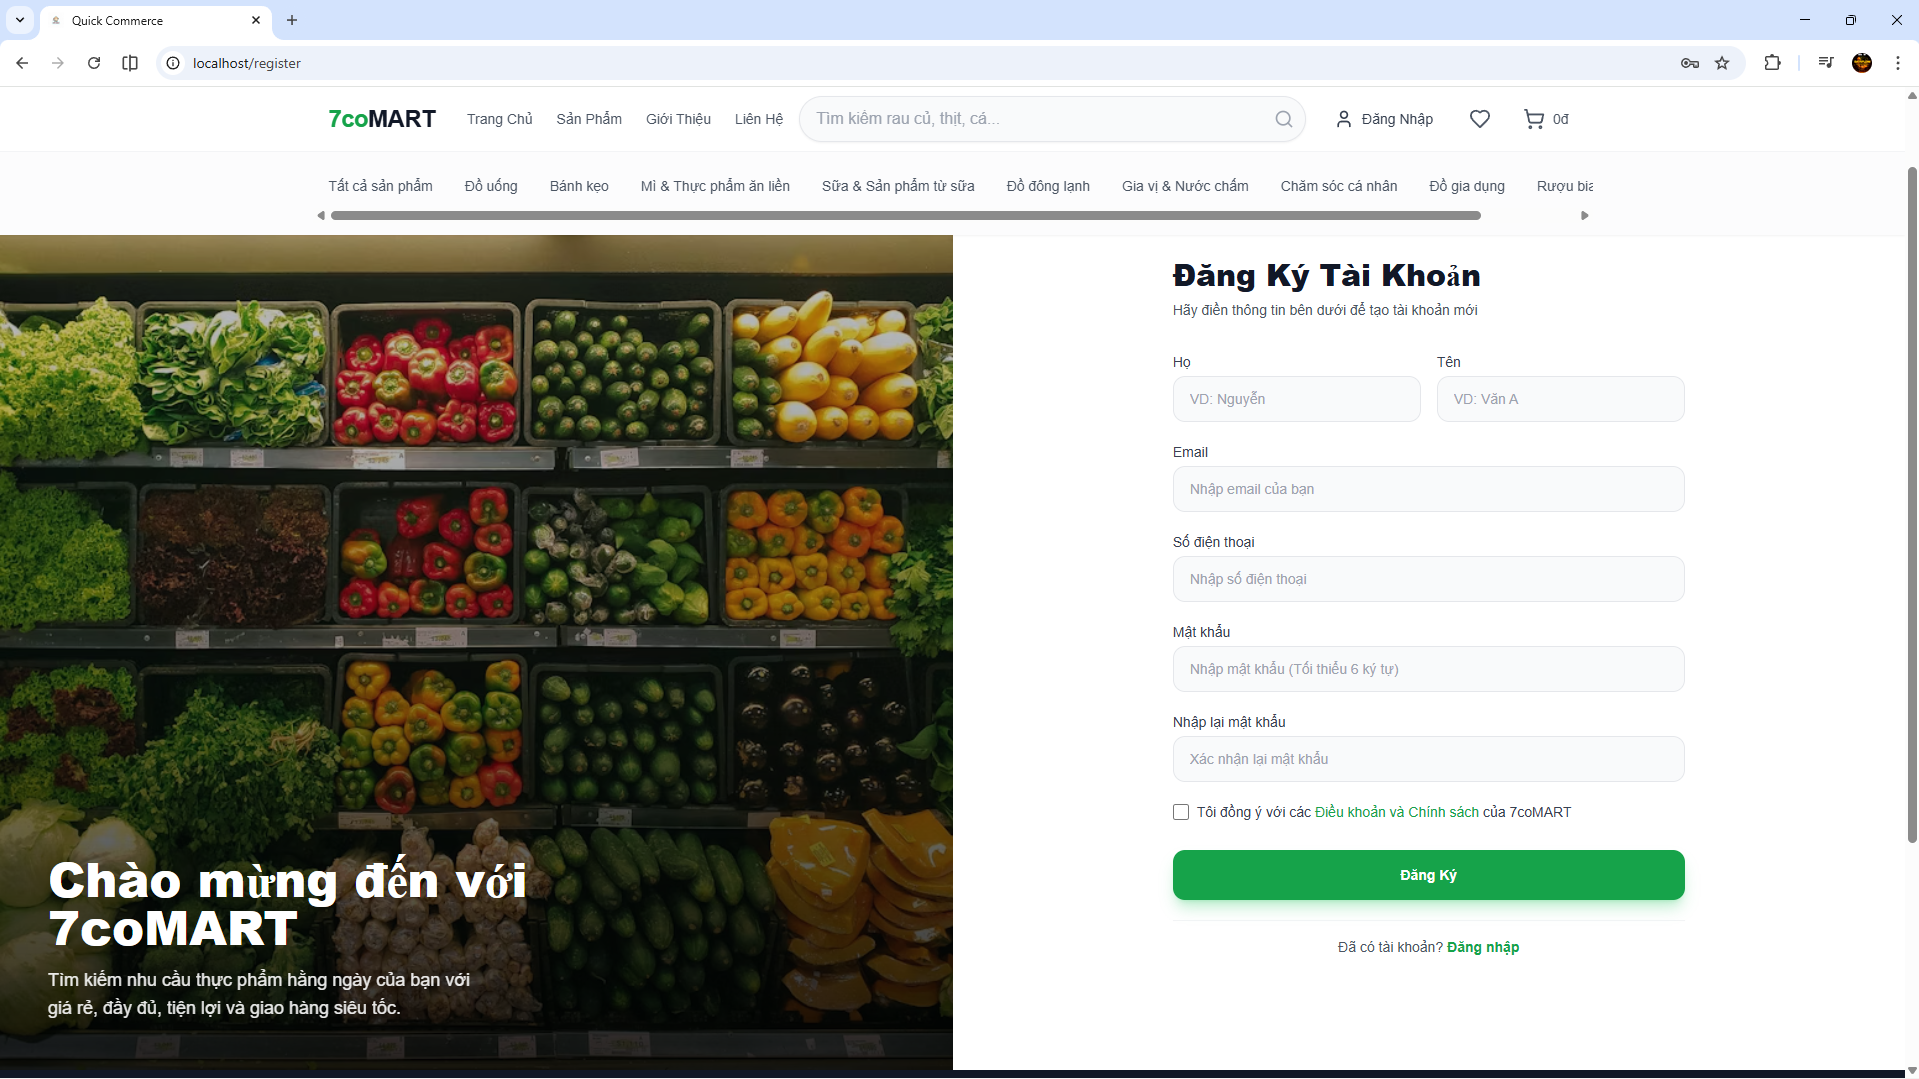
\includegraphics[width=\textwidth]{figs/register.png}
        \caption{Giao diện form Đăng ký tài khoản mới của hệ thống 7coMART}
        \label{fig:register_ui}
    \end{minipage}
    \hfill
    \begin{minipage}{0.48\textwidth}
        \centering
        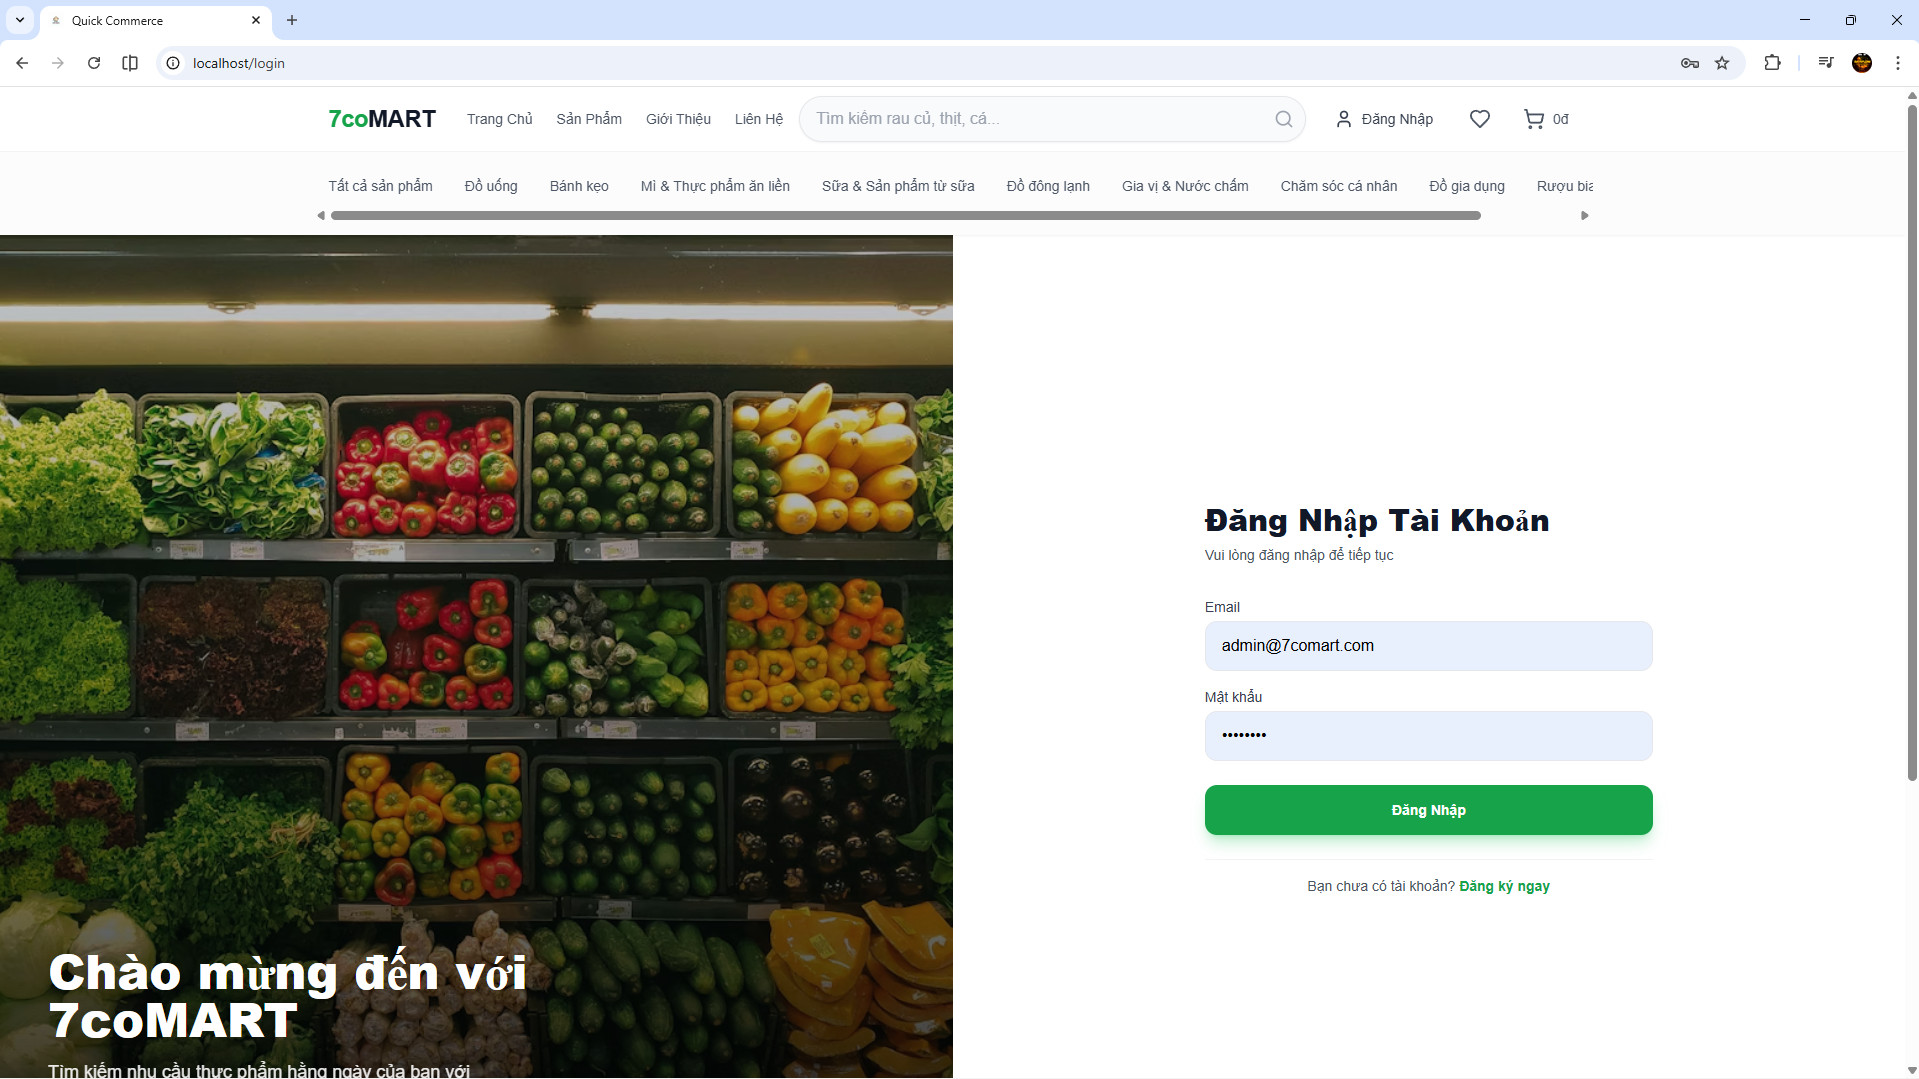
\includegraphics[width=\textwidth]{figs/login.png}
        \caption{Giao diện form Đăng nhập tài khoản của hệ thống 7coMART}
        \label{fig:login_ui}
    \end{minipage}
\end{figure}

Hình \ref{fig:register_ui} và \ref{fig:login_ui} thể hiện sự hoạt động bình thường, đúng nghiệp vụ của các chức năng Xác thực của Khách hàng trong Sprint 1 trước khi tiến hành các kịch bản kiểm tra lỗi.

\begin{figure}[H]
    \centering
    \begin{minipage}{0.48\textwidth}
        \centering
        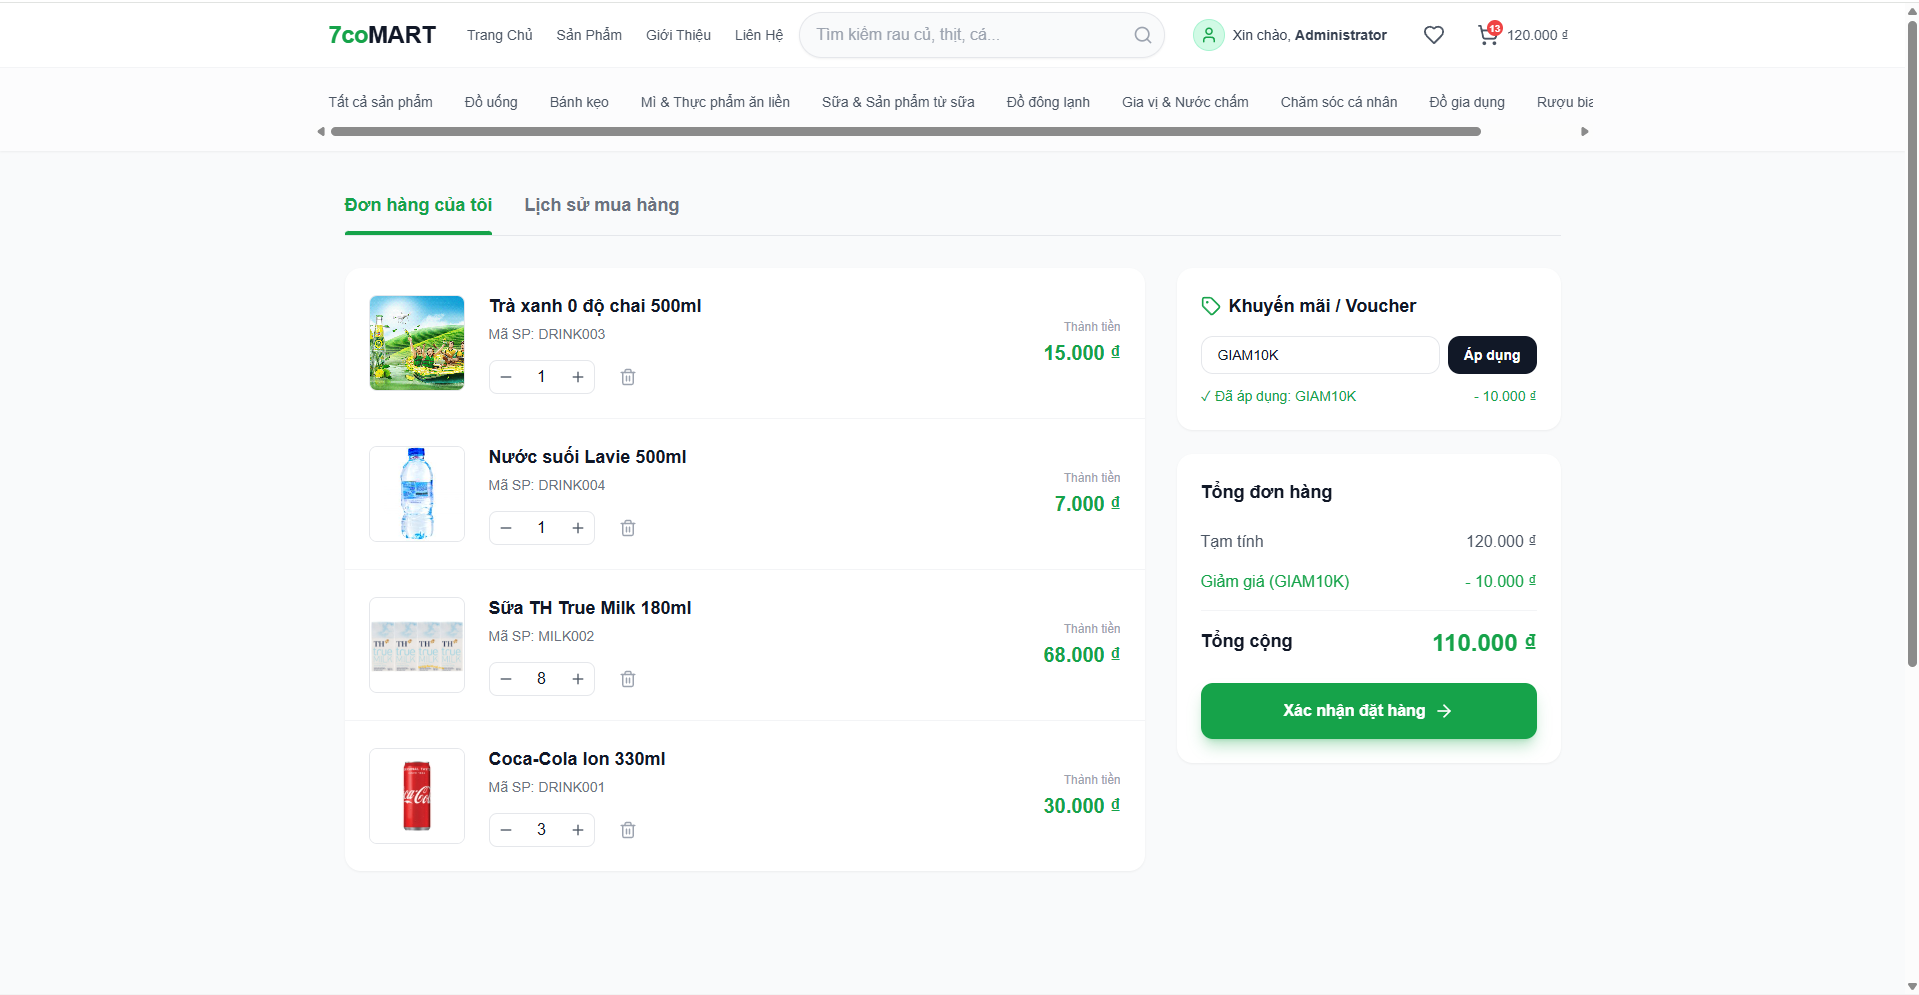
\includegraphics[width=\textwidth]{figs/cart.png}
        \caption{Giao diện Giỏ hàng với các sản phẩm được chọn trong Sprint 2}
        \label{fig:cart_ui}
    \end{minipage}
    \hfill
    \begin{minipage}{0.48\textwidth}
        \centering
        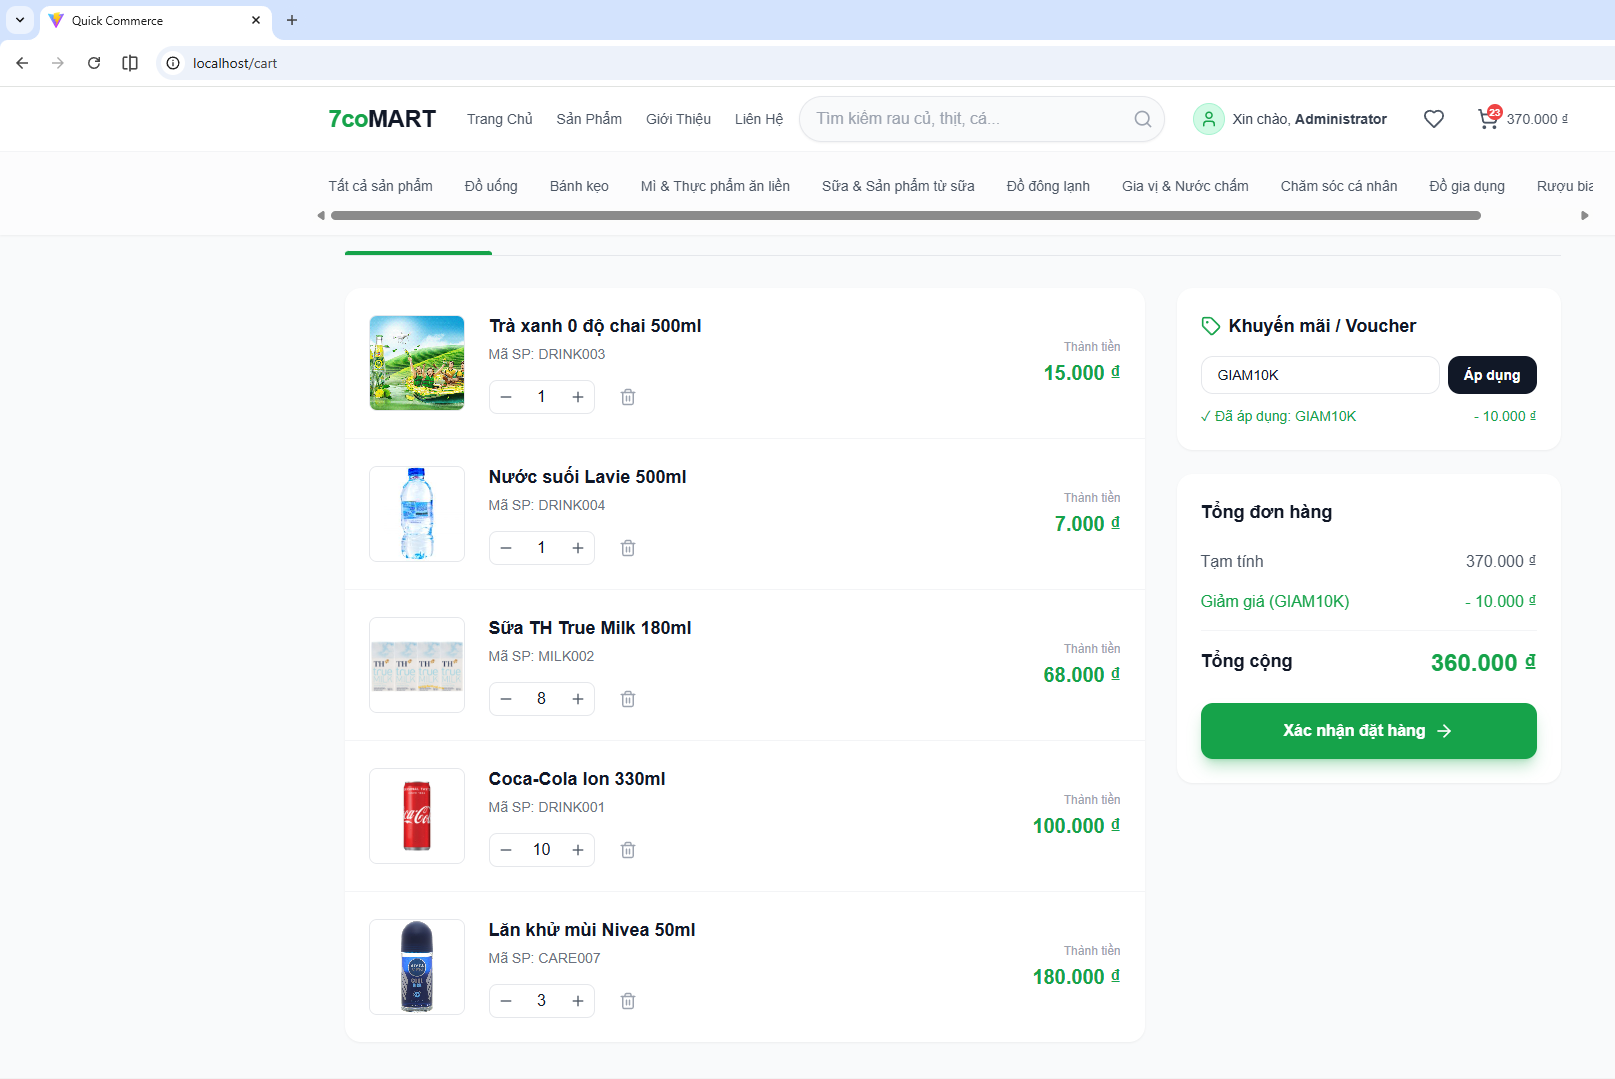
\includegraphics[width=\textwidth]{figs/test_cart_result.png}
        \caption{Giao diện thanh toán và kiểm định logic giỏ hàng}
        \label{fig:cart_result_ui}
    \end{minipage}
\end{figure}

Như được minh họa tại Hình \ref{fig:cart_ui} và \ref{fig:cart_result_ui}, hệ thống giỏ hàng của 7coMART hiển thị chính xác tên sản phẩm, đơn giá, tổng giá tiền tạm tính thời gian thực và cho phép cập nhật số lượng trơn tru đối với các ca kiểm thử hợp lệ.

\section{Quản lý vòng đời lỗi chuyên nghiệp với Mantis Bug Tracker}

\subsection{Sơ đồ vòng đời lỗi trong LaTeX bằng TikZ}
Để duy trì quy trình sửa lỗi nhất quán, nhóm áp dụng sơ đồ chuyển đổi trạng thái lỗi chuẩn của MantisBT. Dưới đây là sơ đồ vòng đời lỗi được vẽ trực tiếp bằng thư viện TikZ sắc nét:

\begin{center}
\begin{tikzpicture}[node distance=2.5cm, auto]
    % Define styles
    \tikzstyle{state} = [rectangle, rounded corners, minimum width=2.5cm, minimum height=1cm, text centered, draw=blue!80, fill=blue!10, thick]
    \tikzstyle{line} = [draw, -latex, thick, blue!80]
    
    % Place nodes
    \node [state] (new) {NEW (Tester phát hiện)};
    \node [state, right of=new, node distance=4.5cm] (assigned) {ASSIGNED (Dev nhận lỗi)};
    \node [state, right of=assigned, node distance=4.5cm] (resolved) {RESOLVED (Đã vá lỗi)};
    \node [state, below of=resolved, node distance=2.5cm] (closed) {CLOSED (Tester đóng lỗi)};
    
    % Draw edges
    \path [line] (new) -- (assigned);
    \path [line] (assigned) -- (resolved);
    \path [line] (resolved) -- (closed);
    \path [line] (resolved) |- node [near end, above] {Re-test Fail} (new);
\end{tikzpicture}
\end{center}

\subsection{Quy trình viết Báo cáo lỗi (Defect Report) chuẩn chỉnh}
Một Báo cáo lỗi chuyên nghiệp trên Mantis bắt buộc phải cung cấp đầy đủ thông tin để Lập trình viên có thể dễ dàng tái hiện lỗi và tiến hành sửa đổi mã nguồn:
\begin{enumerate}
    \item \textbf{Summary (Tiêu đề):} Mô tả cực kỳ ngắn gọn, định danh vị trí lỗi (Ví dụ: \texttt{[Cart API] Lỗi nhập số lượng âm rút tiền hệ thống}).
    \item \textbf{Description (Mô tả chi tiết):} Nêu rõ hành vi không mong muốn của hệ thống và ảnh hưởng của nó.
    \item \textbf{Steps to Reproduce (Các bước tái hiện):} Liệt kê các bước thao tác tuần tự (1, 2, 3...) để bất kỳ ai cũng có thể kích hoạt lại đúng lỗi đó trên máy của mình.
    \item \textbf{Severity (Mức độ nghiêm trọng):} Phân cấp mức độ ảnh hưởng (Block, Crash, Major, Minor).
    \item \textbf{Priority (Độ ưu tiên):} Đánh giá mức độ khẩn cấp cần sửa (Urgent, High, Normal, Low).
\end{enumerate}

\begin{figure}[H]
    \centering
    \begin{tikzpicture}[scale=0.8, every node/.style={transform shape}]
        % Browser border
        \draw[thick, fill=white] (0,0) rectangle (15,9.5);
        % Browser title bar
        \draw[fill=gray!20, thick] (0,8.7) rectangle (15,9.5);
        % Red, yellow, green window controls
        \fill[red] (0.3,9.15) circle (0.12);
        \fill[yellow] (0.7,9.15) circle (0.12);
        \fill[green] (1.1,9.15) circle (0.12);
        % Address bar
        \draw[fill=white, rounded corners=2pt] (2.0,8.85) rectangle (12.0,9.35);
        \node[right] at (2.2,9.1) {\scriptsize \texttt{http://localhost:8089/view\_all\_bug\_page.php}};
        
        % Left Sidebar (MantisBT menu)
        \draw[fill=gray!80, draw=none] (0,0) rectangle (2.5,8.7);
        \node[white, right] at (0.2,8.3) {\small\textbf{MantisBT v2.25}};
        \draw[white!50] (0.2,8.0) -- (2.3,8.0);
        \node[white, right] at (0.3,7.5) {\tiny $\bullet$ Bảng điều khiển};
        \node[white, right] at (0.3,7.0) {\tiny $\bullet$ Xem danh sách lỗi};
        \node[white, right] at (0.3,6.5) {\tiny $\bullet$ Báo cáo lỗi};
        \node[white, right] at (0.3,6.0) {\tiny $\bullet$ Quản lý hệ thống};
        
        % Main Workspace Header
        \node[right] at (2.8,8.2) {\small\textbf{Danh sách sự cố lỗi đã ghi nhận (7coMART)}};
        \draw[gray!30] (2.8,7.8) -- (14.5,7.8);
        
        % Table Header
        \draw[fill=gray!20, draw=gray] (2.8,7.0) rectangle (14.5,7.5);
        \node[right] at (2.9,7.25) {\tiny\textbf{ID}};
        \node[right] at (3.8,7.25) {\tiny\textbf{Danh mục}};
        \node[right] at (5.8,7.25) {\tiny\textbf{Mức độ}};
        \node[right] at (7.2,7.25) {\tiny\textbf{Trạng thái}};
        \node[right] at (8.8,7.25) {\tiny\textbf{Tóm tắt sự cố}};
        
        % Row 1: SQL Injection
        \draw[draw=gray] (2.8,6.2) rectangle (14.5,7.0);
        \node[right] at (2.9,6.6) {\tiny \texttt{0000021}};
        \node[right] at (3.8,6.6) {\tiny Xác thực (Auth)};
        \node[right, fill=red!20, rounded corners=2.5pt] at (5.8,6.6) {\tiny\textbf{Block}};
        \node[right, fill=orange!20, rounded corners=2.5pt] at (7.2,6.6) {\tiny\textbf{New}};
        \node[right] at (8.8,6.6) {\tiny [Login] Lỗ hổng bảo mật SQL Injection tại form Đăng nhập};
        
        % Row 2: Unicode Search
        \draw[draw=gray] (2.8,5.4) rectangle (14.5,6.2);
        \node[right] at (2.9,5.8) {\tiny \texttt{0000022}};
        \node[right] at (3.8,5.8) {\tiny Tìm kiếm (Catalog)};
        \node[right, fill=orange!10, rounded corners=2.5pt] at (5.8,5.8) {\tiny\textbf{Major}};
        \node[right, fill=blue!20, rounded corners=2.5pt] at (7.2,5.8) {\tiny\textbf{Assigned}};
        \node[right] at (8.8,5.8) {\tiny Lỗi 500 Internal Server Error khi tìm tiếng Việt Unicode};
        
        % Row 3: Negative quantity
        \draw[draw=gray] (2.8,4.6) rectangle (14.5,5.4);
        \node[right] at (2.9,5.0) {\tiny \texttt{0000023}};
        \node[right] at (3.8,5.0) {\tiny Giỏ hàng (Cart)};
        \node[right, fill=red!10, rounded corners=2.5pt] at (5.8,5.0) {\tiny\textbf{Critical}};
        \node[right, fill=green!20, rounded corners=2.5pt] at (7.2,5.0) {\tiny\textbf{Resolved}};
        \node[right] at (8.8,5.0) {\tiny Hacker can thiệp sửa đổi số lượng âm giỏ hàng qua HTTP};
        
        % Row 4: Interface small bug
        \draw[draw=gray] (2.8,3.8) rectangle (14.5,4.6);
        \node[right] at (2.9,4.2) {\tiny \texttt{0000024}};
        \node[right] at (3.8,4.2) {\tiny Giao diện (UI)};
        \node[right, fill=gray!20, rounded corners=2.5pt] at (5.8,4.2) {\tiny\textbf{Minor}};
        \node[right, fill=green!20, rounded corners=2.5pt] at (7.2,4.2) {\tiny\textbf{Closed}};
        \node[right] at (8.8,4.2) {\tiny Lỗi tràn viền nút bấm mua sản phẩm nhanh trên mobile};
    \end{tikzpicture}
    \caption{Giao diện bảng điều khiển quản lý và theo dõi lỗi Mantis Bug Tracker của dự án 7coMART}
    \label{fig:mantis_dashboard}
\end{figure}

\textbf{Nhận xét Hệ thống:} Qua giao diện Dashboard tại Hình \ref{fig:mantis_dashboard}, các lỗi được lập chỉ mục khoa học với màu sắc nhận diện trạng thái trực quan, giúp ban quản trị dự án nhanh chóng đánh giá số lượng lỗi tồn đọng và phân phối nhiệm vụ vá lỗi hiệu quả cho các Lập trình viên.

\section{Thống kê và Chi tiết một số lỗi (Bugs) tiêu biểu}
Dưới đây là chi tiết 03 lỗi nghiêm trọng thực tế được Tester phát hiện trên hệ thống 7coMART và ghi nhận chuẩn xác lên hệ thống ticket Mantis Bug Tracker.

\subsection{Bug 1: Lỗ hổng bảo mật SQL Injection tại Form Đăng nhập}
\begin{itemize}
    \item \textbf{Mã Ticket Mantis:} \texttt{\#0000021}
    \item \textbf{Mô-đun ảnh hưởng:} Xác thực (Authentication / Login API)
    \item \textbf{Mức độ nghiêm trọng:} \textbf{Block (Phong tỏa hệ thống)} - Cho phép vượt qua cơ chế bảo mật đăng nhập.
    \item \textbf{Các bước tái hiện:}
    \begin{enumerate}
        \item Truy cập giao diện Đăng nhập tại địa chỉ \url{http://localhost/login}.
        \item Tại ô email nhập chuỗi ký tự tấn công: \texttt{' OR 1=1 --}
        \item Tại ô mật khẩu nhập giá trị bất kỳ: \texttt{xyz123}
        \item Bấm nút ``Đăng nhập''.
    \end{enumerate}
    \item \textbf{Kết quả thực tế:} Hệ thống bỏ qua bước kiểm tra mật khẩu, tự động đăng nhập thẳng vào tài khoản Quản trị viên (Admin) cấp cao nhất do backend thực thi nối chuỗi SQL thô trực tiếp không qua tham số hóa.
    \item \textbf{Kết quả mong đợi:} Hệ thống phát hiện dữ liệu nhập vào không hợp lệ, từ chối đăng nhập và đưa ra cảnh báo lỗi bảo mật hoặc tài khoản sai.
\end{itemize}

\begin{figure}[H]
    \centering
    \begin{tikzpicture}[scale=0.8, every node/.style={transform shape}]
        % Browser frame
        \draw[thick, fill=white] (0,0) rectangle (15,9.5);
        \draw[fill=gray!20, thick] (0,8.7) rectangle (15,9.5);
        \fill[red] (0.3,9.1) circle (0.12);
        \fill[yellow] (0.7,9.1) circle (0.12);
        \fill[green] (1.1,9.1) circle (0.12);
        \draw[fill=white, rounded corners=2pt] (2.0,8.85) rectangle (12.0,9.35);
        \node[right] at (2.2,9.1) {\scriptsize \texttt{http://localhost:8089/view.php?id=21}};
        
        % Left Sidebar (MantisBT menu)
        \draw[fill=gray!80, draw=none] (0,0) rectangle (2.5,8.7);
        \node[white, right] at (0.3,8.0) {\tiny $\bullet$ Xem danh sách lỗi};
        \node[white, right] at (0.3,7.5) {\tiny $\bullet$ Báo cáo sự cố};
        
        % Main Workspace Header
        \node[right] at (2.8,8.2) {\small\textbf{Xem chi tiết sự cố: \#0000021}};
        \draw[gray!30] (2.8,7.9) -- (14.5,7.9);
        
        % Ticket Details Grid
        \draw[draw=gray, fill=gray!5] (2.8,4.0) rectangle (14.5,7.6);
        % Headers
        \node[right] at (2.9,7.3) {\tiny\textbf{ID:}}; 
        \node[right] at (5.2,7.3) {\tiny 0000021};
        \node[right] at (8.0,7.3) {\tiny\textbf{Danh mục:}}; 
        \node[right] at (10.2,7.3) {\tiny Xác thực (Auth)};
        \draw[gray!20] (2.8,7.0) -- (14.5,7.0);
        
        \node[right] at (2.9,6.7) {\tiny\textbf{Mức độ nghiêm trọng:}}; 
        \node[right, fill=red!20, rounded corners=2pt] at (5.2,6.7) {\tiny\textbf{Block}};
        \node[right] at (8.0,6.7) {\tiny\textbf{Độ ưu tiên:}}; 
        \node[right] at (10.2,6.7) {\tiny Khẩn cấp (Urgent)};
        \draw[gray!20] (2.8,6.4) -- (14.5,6.4);
        
        \node[right] at (2.9,6.1) {\tiny\textbf{Người báo cáo:}}; 
        \node[right] at (5.2,6.1) {\tiny Đinh Minh Đức (Reporter)};
        \node[right] at (8.0,6.1) {\tiny\textbf{Trạng thái:}}; 
        \node[right, fill=orange!20, rounded corners=2pt] at (10.2,6.1) {\tiny\textbf{New}};
        \draw[gray!20] (2.8,5.8) -- (14.5,5.8);
        
        \node[right] at (2.9,5.5) {\tiny\textbf{Tóm tắt:}}; 
        \node[right] at (4.5,5.5) {\tiny\textbf{[Login API] Lỗ hổng SQL Injection tại Form đăng nhập}};
        \draw[gray!20] (2.8,5.2) -- (14.5,5.2);
        
        \node[right] at (2.9,4.7) {\tiny\textbf{Mô tả:}};
        \node[right] at (4.5,4.8) {\tiny Nhập chuỗi độc hại \texttt{' OR 1=1 --} vào ô email cho phép vượt qua};
        \node[right] at (4.5,4.4) {\tiny kiểm định bảo mật mật khẩu và chiếm quyền quản trị Admin.};
        
        % Steps to reproduce
        \draw[draw=gray] (2.8,1.0) rectangle (14.5,3.6);
        \node[right] at (2.9,3.2) {\tiny\textbf{Các bước tái hiện:}};
        \node[right] at (3.1,2.8) {\tiny 1. Truy cập \url{http://localhost/login}};
        \node[right] at (3.1,2.4) {\tiny 2. Nhập email: \texttt{' OR 1=1 --}};
        \node[right] at (3.1,2.0) {\tiny 3. Nhập mật khẩu tùy ý: \texttt{xyz}};
        \node[right] at (3.1,1.6) {\tiny 4. Bấm đăng nhập $\rightarrow$ Đăng nhập thành công và chuyển hướng về tài khoản Admin.};
    \end{tikzpicture}
    \caption{Chi tiết ticket lỗi bảo mật SQL Injection trên form Đăng nhập được ghi nhận trên MantisBT}
    \label{fig:bug_sqli}
\end{figure}

\textbf{Phân tích rủi ro:} Lỗi được chỉ ra tại Hình \ref{fig:bug_sqli} là lỗ hổng bảo mật cực kỳ nguy hại. Một kẻ tấn công ngoài mạng có thể dễ dàng kiểm soát toàn bộ cơ sở dữ liệu khách hàng, sửa đổi giá tiền sản phẩm hoặc chiếm quyền quản trị tối cao của 7coMART mà không cần bất cứ kiến thức mật khẩu nào.

\subsection{Bug 2: Lỗi 500 Internal Server Error khi tìm kiếm từ khóa tiếng Việt chứa Unicode}
\begin{itemize}
    \item \textbf{Mã Ticket Mantis:} \texttt{\#0000022}
    \item \textbf{Mô-đun ảnh hưởng:} Tra cứu sản phẩm (Catalog Search API)
    \item \textbf{Mức độ nghiêm trọng:} \textbf{Major (Lỗi lớn)} - Làm tê liệt chức năng tìm kiếm sản phẩm của người dùng Việt.
    \item \textbf{Các bước tái hiện:}
    \begin{enumerate}
        \item Truy cập trang chủ bán hàng \url{http://localhost}.
        \item Gõ từ khóa tìm kiếm có dấu: ``sữa tươi'' hoặc ``mì ăn liền'' vào ô tìm kiếm.
        \item Nhấn phím Enter hoặc nút Tìm kiếm.
    \end{enumerate}
    \item \textbf{Kết quả thực tế:} Giao diện quay vô tận, Console báo lỗi mạng, gọi API trả về mã lỗi \texttt{500 Internal Server Error} từ backend FastAPI do cơ sở dữ liệu gặp sự cố đối chiếu bảng mã Unicode của PostgreSQL.
    \item \textbf{Kết quả mong đợi:} Hệ thống hiển thị danh sách các sản phẩm sữa tươi hoặc mì gói bình thường, xử lý trơn tru bảng mã tiếng Việt UTF-8.
\end{itemize}

\begin{figure}[H]
    \centering
    \begin{tikzpicture}[scale=0.8, every node/.style={transform shape}]
        % Browser frame
        \draw[thick, fill=white] (0,0) rectangle (15,9.5);
        \draw[fill=gray!20, thick] (0,8.7) rectangle (15,9.5);
        \fill[red] (0.3,9.1) circle (0.12);
        \fill[yellow] (0.7,9.1) circle (0.12);
        \fill[green] (1.1,9.1) circle (0.12);
        \draw[fill=white, rounded corners=2pt] (2.0,8.85) rectangle (12.0,9.35);
        \node[right] at (2.2,9.1) {\scriptsize \texttt{http://localhost:8089/view.php?id=22}};
        
        % Left Sidebar (MantisBT menu)
        \draw[fill=gray!80, draw=none] (0,0) rectangle (2.5,8.7);
        \node[white, right] at (0.3,8.0) {\tiny $\bullet$ Xem danh sách lỗi};
        
        % Main Workspace Header
        \node[right] at (2.8,8.2) {\small\textbf{Xem chi tiết sự cố: \#0000022}};
        \draw[gray!30] (2.8,7.9) -- (14.5,7.9);
        
        % Ticket Details Grid
        \draw[draw=gray, fill=gray!5] (2.8,4.0) rectangle (14.5,7.6);
        % Headers
        \node[right] at (2.9,7.3) {\tiny\textbf{ID:}}; 
        \node[right] at (5.2,7.3) {\tiny 0000022};
        \node[right] at (8.0,7.3) {\tiny\textbf{Danh mục:}}; 
        \node[right] at (10.2,7.3) {\tiny Tra cứu (Search)};
        \draw[gray!20] (2.8,7.0) -- (14.5,7.0);
        
        \node[right] at (2.9,6.7) {\tiny\textbf{Mức độ nghiêm trọng:}}; 
        \node[right, fill=orange!20, rounded corners=2pt] at (5.2,6.7) {\tiny\textbf{Major}};
        \node[right] at (8.0,6.7) {\tiny\textbf{Độ ưu tiên:}}; 
        \node[right] at (10.2,6.7) {\tiny Cao (High)};
        \draw[gray!20] (2.8,6.4) -- (14.5,6.4);
        
        \node[right] at (2.9,6.1) {\tiny\textbf{Người báo cáo:}}; 
        \node[right] at (5.2,6.1) {\tiny Nguyễn Quang Huy (Reporter)};
        \node[right] at (8.0,6.1) {\tiny\textbf{Trạng thái:}}; 
        \node[right, fill=blue!20, rounded corners=2pt] at (10.2,6.1) {\tiny\textbf{Assigned}};
        \draw[gray!20] (2.8,5.8) -- (14.5,5.8);
        
        \node[right] at (2.9,5.5) {\tiny\textbf{Tóm tắt:}}; 
        \node[right] at (4.5,5.5) {\tiny\textbf{[Search API] Lỗi 500 Internal Server Error khi tìm tiếng Việt Unicode}};
        \draw[gray!20] (2.8,5.2) -- (14.5,5.2);
        
        \node[right] at (2.9,4.7) {\tiny\textbf{Mô tả:}};
        \node[right] at (4.5,4.8) {\tiny Nhập từ khóa có dấu tiếng Việt như ``sữa tươi'' gây crash API};
        \node[right] at (4.5,4.4) {\tiny và trả về mã lỗi 500 Internal Server Error do đối chiếu cơ sở dữ liệu.};
        
        % Steps to reproduce
        \draw[draw=gray] (2.8,1.0) rectangle (14.5,3.6);
        \node[right] at (2.9,3.2) {\tiny\textbf{Các bước tái hiện:}};
        \node[right] at (3.1,2.8) {\tiny 1. Truy cập \url{http://localhost}};
        \node[right] at (3.1,2.4) {\tiny 2. Gõ vào ô tìm kiếm: ``sữa tươi''};
        \node[right] at (3.1,2.0) {\tiny 3. Bấm Tìm kiếm};
        \node[right] at (3.1,1.6) {\tiny 4. Hệ thống báo lỗi kết nối mạng (500) và crash giao diện tìm kiếm.};
    \end{tikzpicture}
    \caption{Chi tiết ticket lỗi Unicode khi tìm kiếm tiếng Việt có dấu được ghi nhận trên MantisBT}
    \label{fig:bug_unicode}
\end{figure}

\textbf{Phân tích rủi ro:} Chức năng tìm kiếm sản phẩm bị tê liệt hoàn toàn khi nhập tiếng Việt có dấu (Hình \ref{fig:bug_unicode}) gây cản trở nghiêm trọng cho trải nghiệm người dùng, vì đại đa số khách hàng tại Việt Nam đều có thói quen tìm kiếm sản phẩm có dấu tiếng Việt chuẩn.

\subsection{Bug 3: Tấn công thay đổi gói tin sửa đổi số lượng sản phẩm âm trong Giỏ hàng}
\begin{itemize}
    \item \textbf{Mã Ticket Mantis:} \texttt{\#0000023}
    \item \textbf{Mô-đun ảnh hưởng:} Giỏ hàng (Cart API)
    \item \textbf{Mức độ nghiêm trọng:} \textbf{Critical (Khẩn cấp)} - Gây tổn thất tài chính nghiêm trọng cho cửa hàng trực tuyến.
    \item \textbf{Các bước tái hiện:}
    \begin{enumerate}
        \item Thêm 01 sản phẩm bánh ngọt giá 50.000 VNĐ vào giỏ hàng.
        \item Sử dụng phần mềm bắt gói tin (Fiddler/Burp Suite) chặn cuộc gọi HTTP POST API gửi tới endpoint \texttt{/api/v1/cart/items}.
        \item Sửa đổi tham số số lượng trong JSON Body từ \texttt{"quantity": 1} thành \texttt{"quantity": -5}.
        \item Thả gói tin cho truyền tiếp tới server backend FastAPI.
    \end{enumerate}
    \item \textbf{Kết quả thực tế:} API trả về mã \texttt{200 OK}, giỏ hàng ghi nhận số lượng bánh ngọt là -5 chiếc, khiến tổng giá tiền của đơn hàng bị âm thành \texttt{-250.000 VNĐ}, cho phép người dùng lách luật rút tiền ngược khi thanh toán.
    \item \textbf{Kết quả mong đợi:} Backend FastAPI bắt buộc phải chặn gói tin ở mức API, báo lỗi validation số lượng không được nhỏ hơn 1 và trả về mã \texttt{422 Unprocessable Entity}.
\end{itemize}

\begin{figure}[H]
    \centering
    \begin{tikzpicture}[scale=0.8, every node/.style={transform shape}]
        % Browser frame
        \draw[thick, fill=white] (0,0) rectangle (15,9.5);
        \draw[fill=gray!20, thick] (0,8.7) rectangle (15,9.5);
        \fill[red] (0.3,9.1) circle (0.12);
        \fill[yellow] (0.7,9.1) circle (0.12);
        \fill[green] (1.1,9.1) circle (0.12);
        \draw[fill=white, rounded corners=2pt] (2.0,8.85) rectangle (12.0,9.35);
        \node[right] at (2.2,9.1) {\scriptsize \texttt{http://localhost:8089/view.php?id=23}};
        
        % Left Sidebar (MantisBT menu)
        \draw[fill=gray!80, draw=none] (0,0) rectangle (2.5,8.7);
        \node[white, right] at (0.3,8.0) {\tiny $\bullet$ Xem danh sách lỗi};
        
        % Main Workspace Header
        \node[right] at (2.8,8.2) {\small\textbf{Xem chi tiết sự cố: \#0000023}};
        \draw[gray!30] (2.8,7.9) -- (14.5,7.9);
        
        % Ticket Details Grid
        \draw[draw=gray, fill=gray!5] (2.8,4.0) rectangle (14.5,7.6);
        % Headers
        \node[right] at (2.9,7.3) {\tiny\textbf{ID:}}; 
        \node[right] at (5.2,7.3) {\tiny 0000023};
        \node[right] at (8.0,7.3) {\tiny\textbf{Danh mục:}}; 
        \node[right] at (10.2,7.3) {\tiny Giỏ hàng (Cart)};
        \draw[gray!20] (2.8,7.0) -- (14.5,7.0);
        
        \node[right] at (2.9,6.7) {\tiny\textbf{Mức độ nghiêm trọng:}}; 
        \node[right, fill=red!15, rounded corners=2pt] at (5.2,6.7) {\tiny\textbf{Critical}};
        \node[right] at (8.0,6.7) {\tiny\textbf{Độ ưu tiên:}}; 
        \node[right] at (10.2,6.7) {\tiny Khẩn cấp (Urgent)};
        \draw[gray!20] (2.8,6.4) -- (14.5,6.4);
        
        \node[right] at (2.9,6.1) {\tiny\textbf{Người báo cáo:}}; 
        \node[right] at (5.2,6.1) {\tiny Nguyễn Công Thành (Reporter)};
        \node[right] at (8.0,6.1) {\tiny\textbf{Trạng thái:}}; 
        \node[right, fill=green!20, rounded corners=2pt] at (10.2,6.1) {\tiny\textbf{Resolved}};
        \draw[gray!20] (2.8,5.8) -- (14.5,5.8);
        
        \node[right] at (2.9,5.5) {\tiny\textbf{Tóm tắt:}}; 
        \node[right] at (4.5,5.5) {\tiny\textbf{[Cart API] Hacker can thiệp sửa đổi số lượng âm giỏ hàng qua HTTP Request}};
        \draw[gray!20] (2.8,5.2) -- (14.5,5.2);
        
        \node[right] at (2.9,4.7) {\tiny\textbf{Mô tả:}};
        \node[right] at (4.5,4.8) {\tiny Can thiệp HTTP API POST bằng Burp Suite để gửi tham số số lượng};
        \node[right] at (4.5,4.4) {\tiny âm. Backend chấp nhận và trừ tiền hóa đơn thành số lượng âm.};
        
        % Steps to reproduce
        \draw[draw=gray] (2.8,1.0) rectangle (14.5,3.6);
        \node[right] at (2.9,3.2) {\tiny\textbf{Các bước tái hiện:}};
        \node[right] at (3.1,2.8) {\tiny 1. Thêm 1 sản phẩm bánh ngọt giá 50k vào giỏ hàng.};
        \node[right] at (3.1,2.4) {\tiny 2. Chặn HTTP request POST đến \texttt{/api/v1/cart/items} bằng Burp Suite.};
        \node[right] at (3.1,2.0) {\tiny 3. Thay đổi tham số JSON: \texttt{"quantity": -5}};
        \node[right] at (3.1,1.6) {\tiny 4. Báo gửi thành công $\rightarrow$ Giỏ hàng lưu số lượng -5 và giá âm -250k.};
    \end{tikzpicture}
    \caption{Chi tiết ticket lỗi can thiệp sửa đổi số lượng sản phẩm âm trong giỏ hàng được ghi nhận trên MantisBT}
    \label{fig:bug_negative}
\end{figure}

\textbf{Phân tích rủi ro:} Lỗ hổng logic nghiệp vụ tại Hình \ref{fig:bug_negative} cho thấy sự thiếu sót nghiêm trọng trong kiểm tra dữ liệu biên đầu vào tại backend. Kẻ gian lợi dụng lỗ hổng này có thể tạo các đơn hàng giá trị âm khổng lồ để gian lận tiền hoặc gây hỗn loạn dữ liệu kế toán kho của 7coMART.